\subsection{sacabench construct}
\label{framework:cli:sacabench-construct}

{
\begin{wrapfigure}[30]{R}[5mm]{.5\textwidth}
    \vspace{-1.5\baselineskip}
    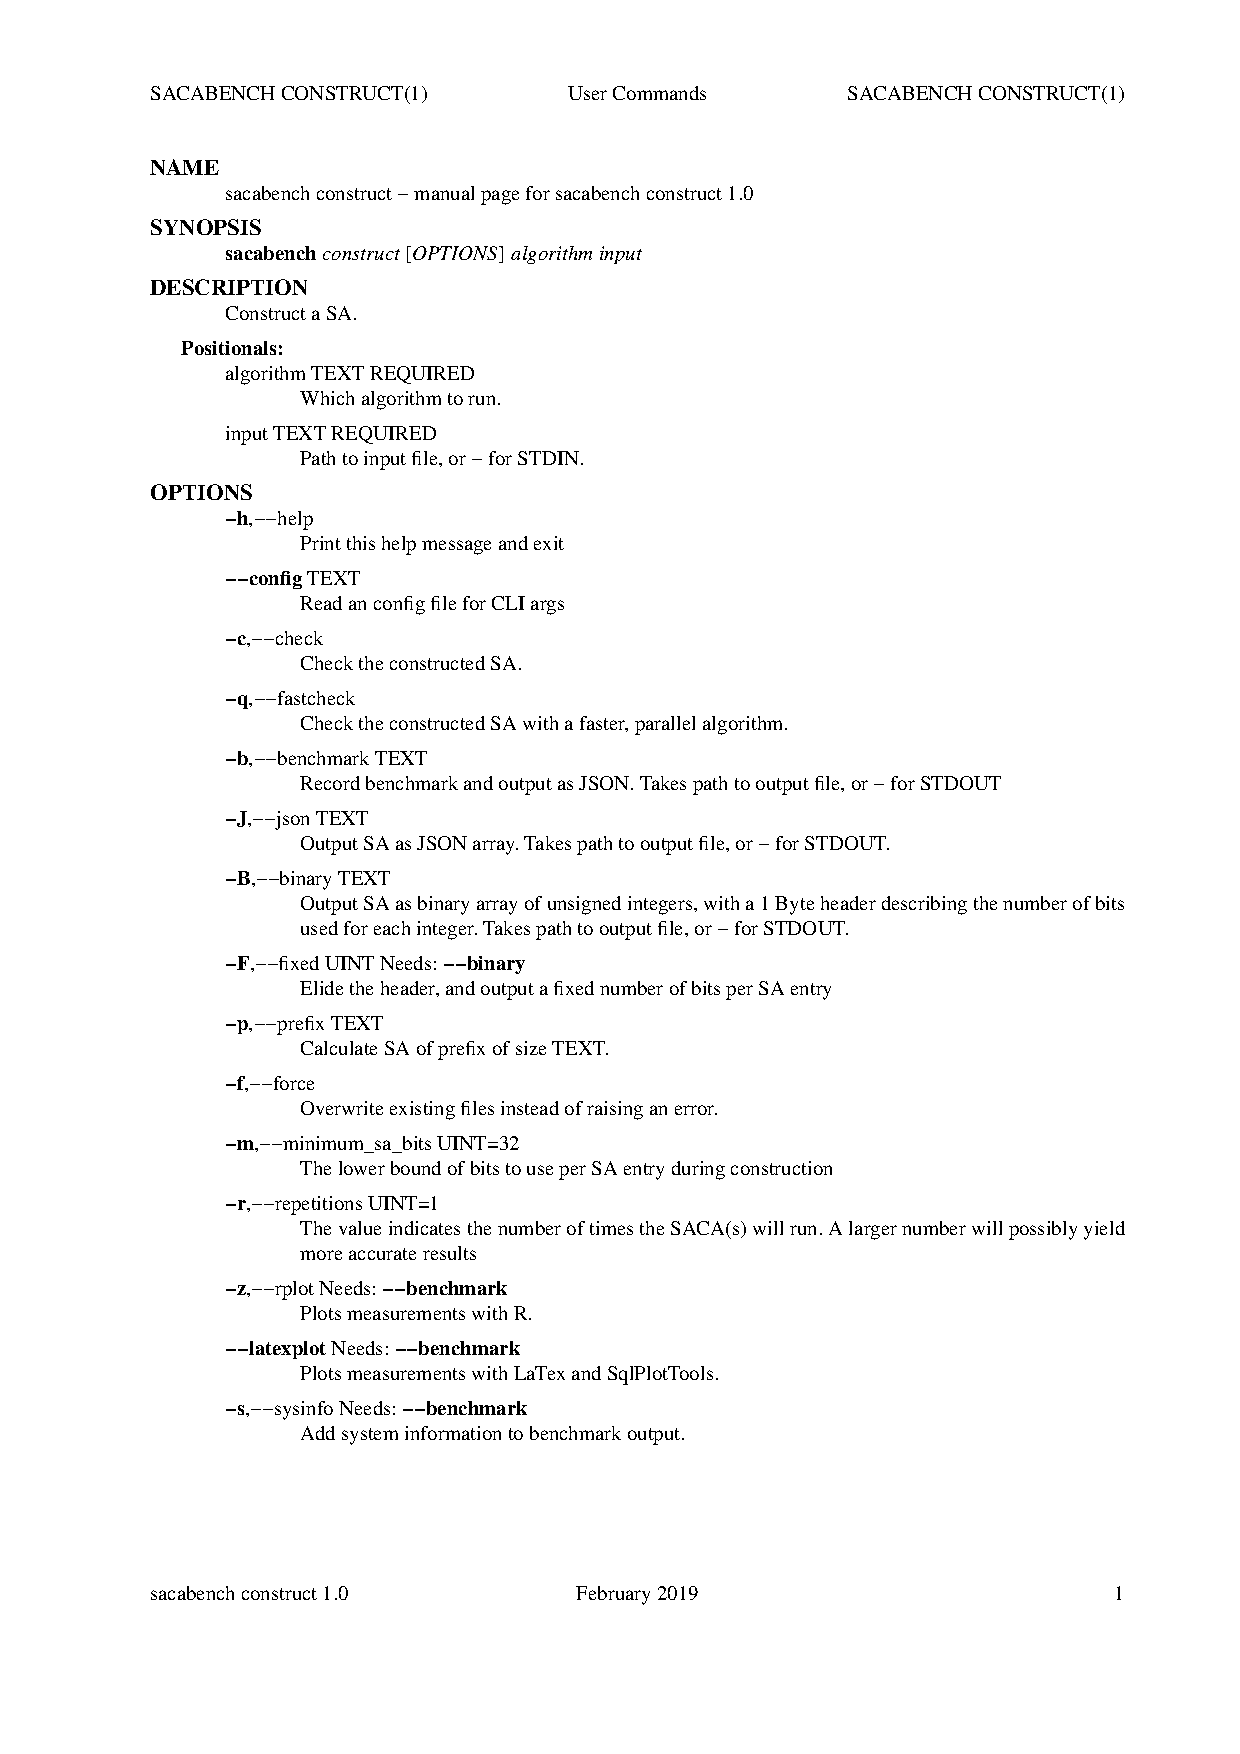
\includegraphics[page=1, viewport=0cm 32.8cm 20.5cm 68.5cm, clip, width=.5\textwidth]{{kapitel/3_framework/cli/sacabench-construct/sacabench-construct}.pdf}\\
    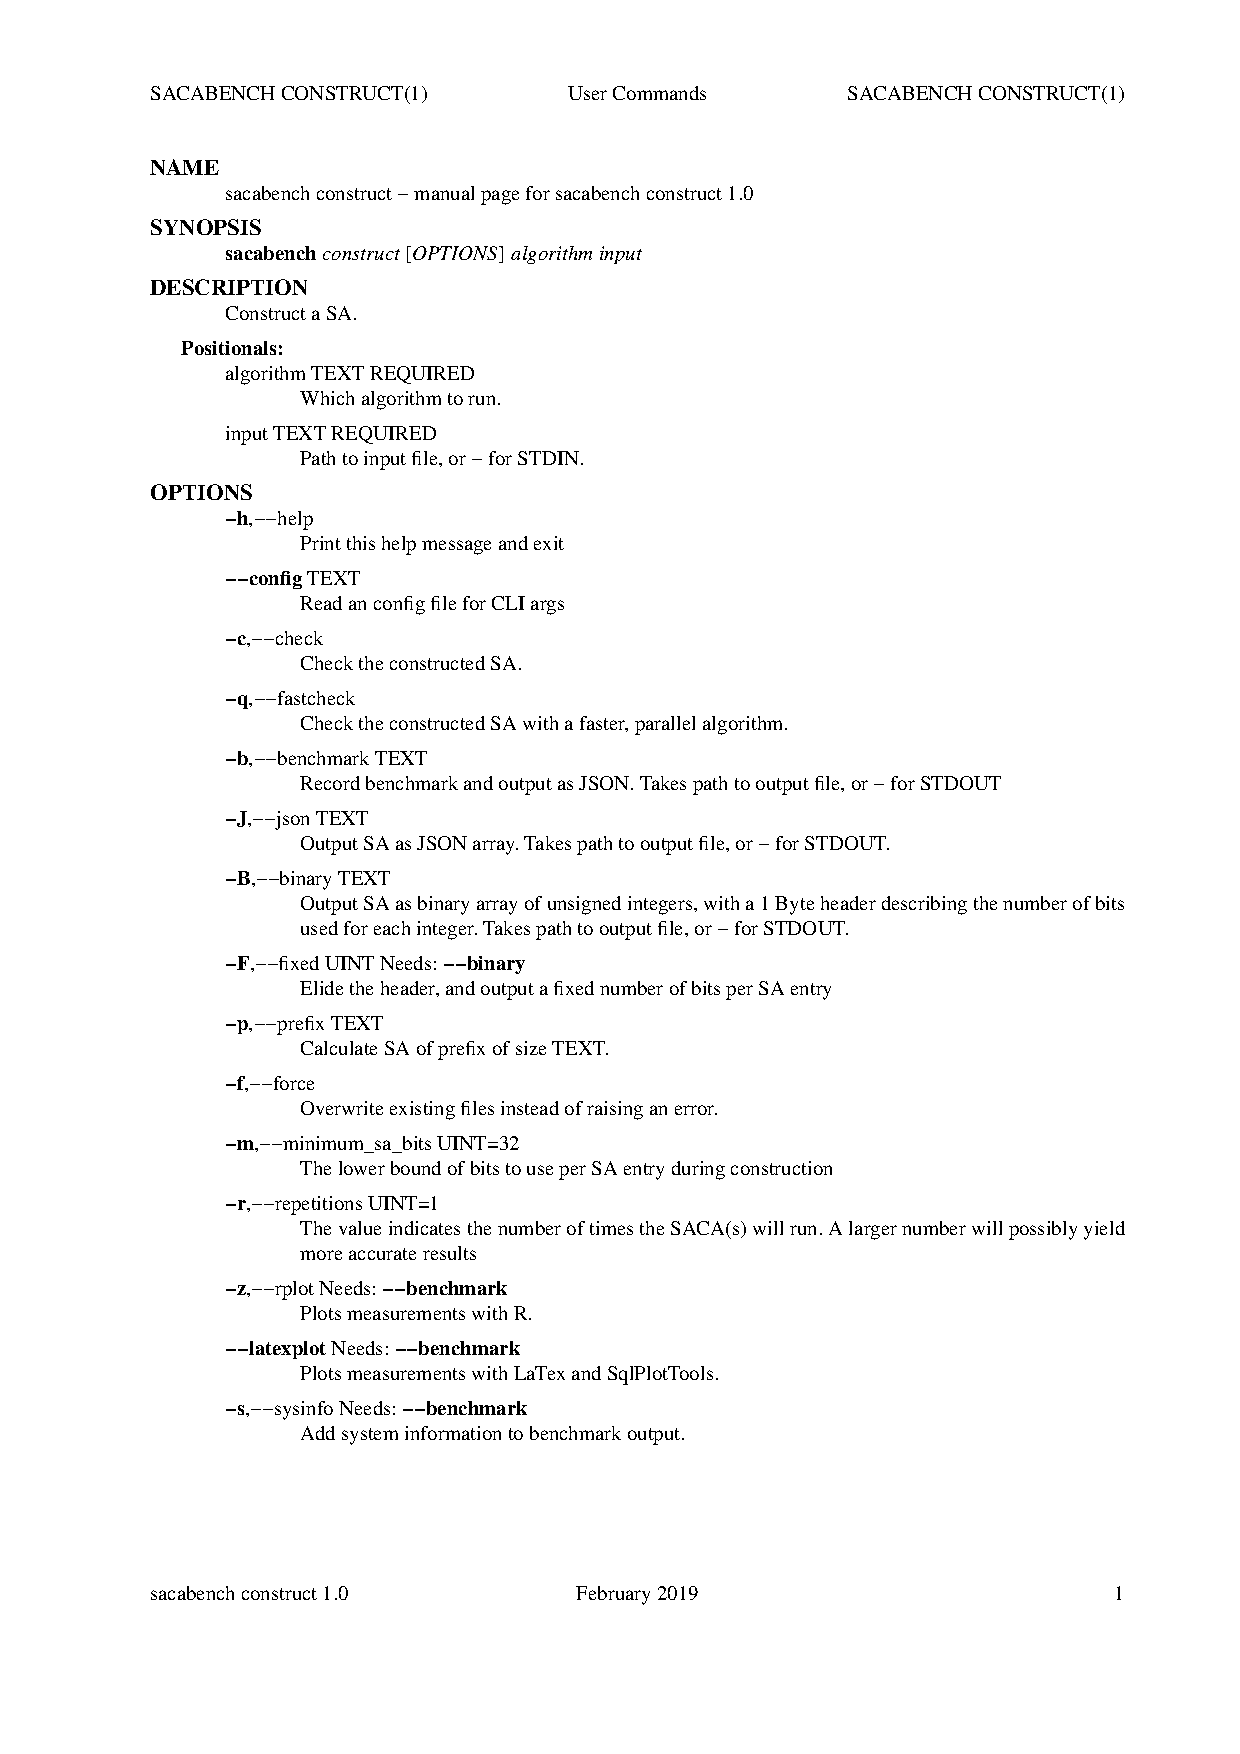
\includegraphics[page=1, viewport=0cm 25cm 20.5cm 26.3cm, clip, width=.5\textwidth]{{kapitel/3_framework/cli/sacabench-construct/sacabench-construct}.pdf}\\
    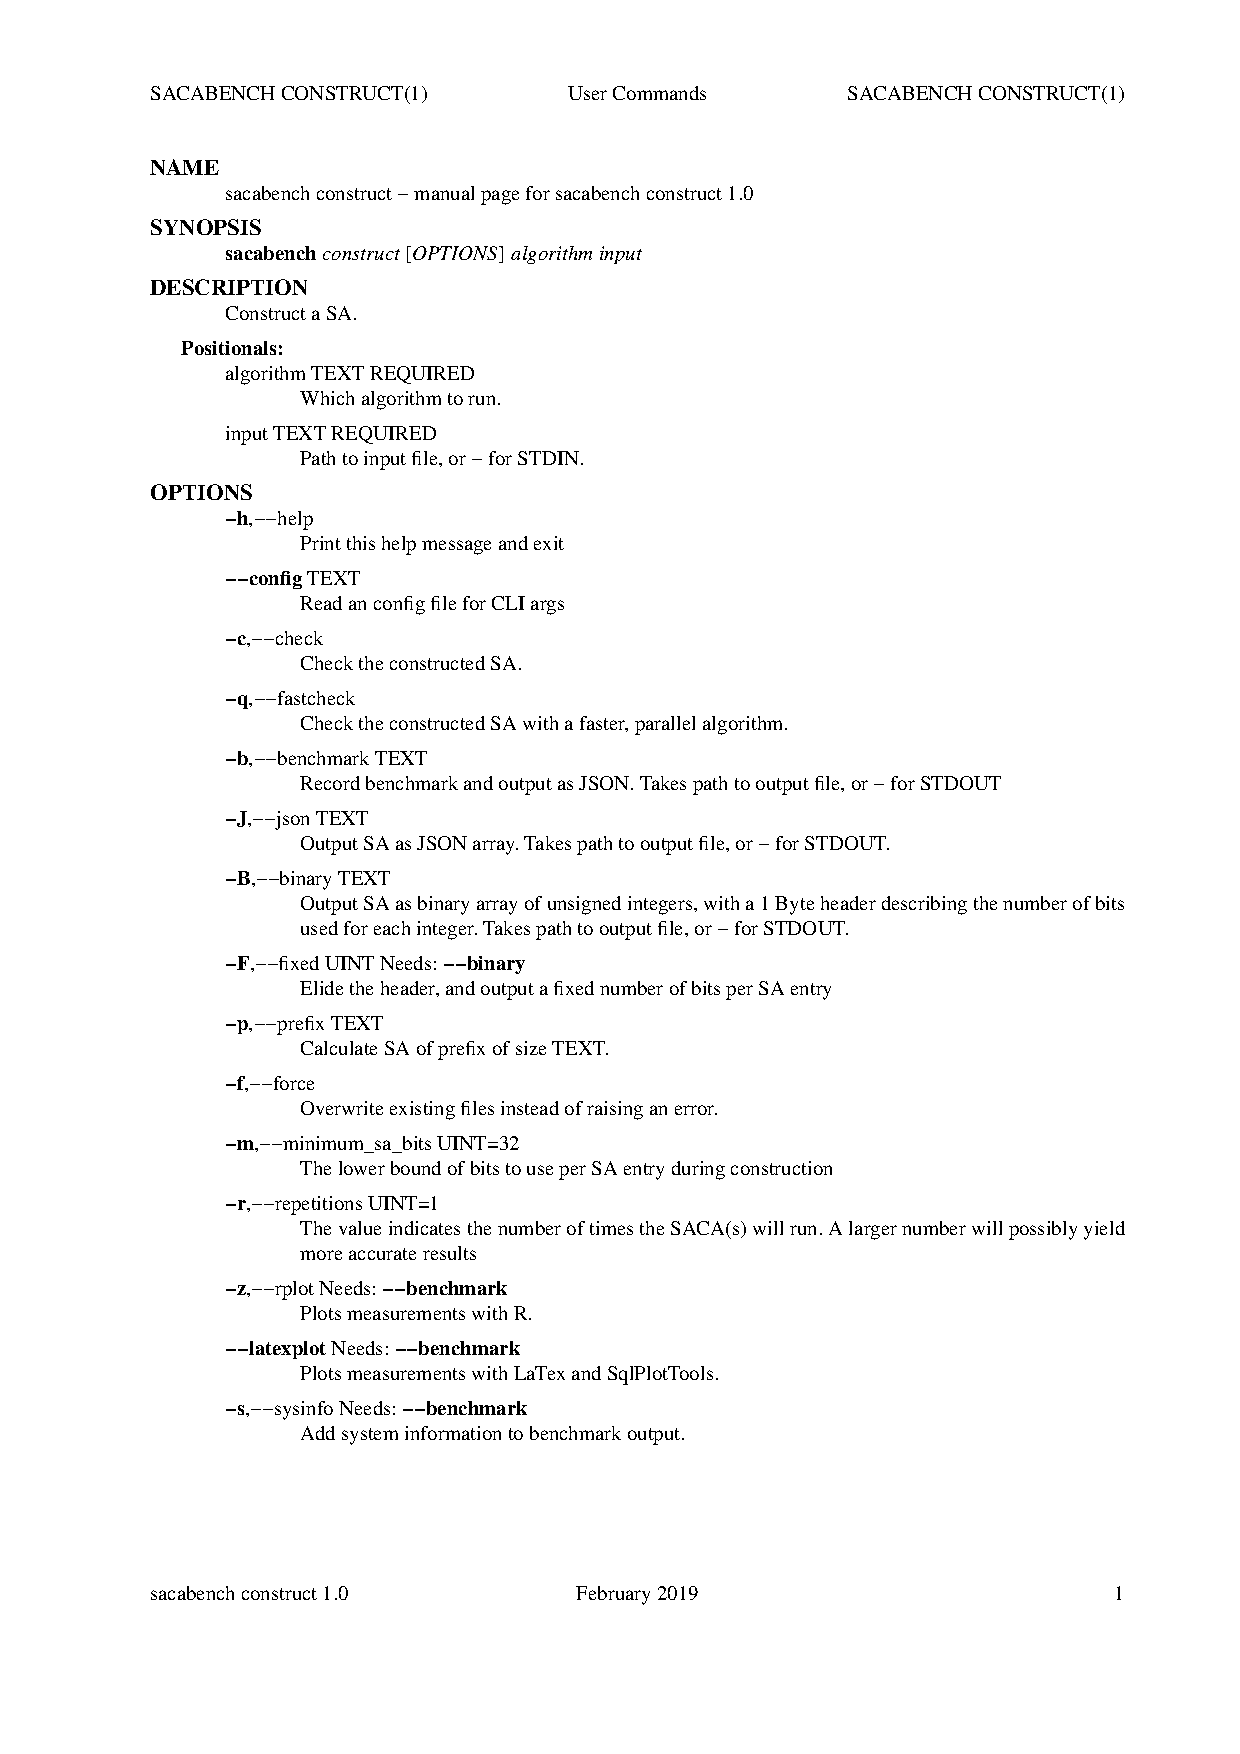
\includegraphics[page=1, viewport=0cm 0cm 20.5cm 1.5cm, clip, width=.5\textwidth]{{kapitel/3_framework/cli/sacabench-construct/sacabench-construct}.pdf}
    \caption{Gekürzte Ausgabe von \texttt{man sacabench construct}.}
    \label{manpage:sacabench-construct}
\end{wrapfigure}

Mit dem Befehl \texttt{sacabench construct} kann ein ausgewählter Algorithmus ausgeführt werden. 
\par
Der auszuführende Algorithmus wird dabei durch sein Kürzel bestimmt, wie es bei \termfont{sacabench list} angegeben ist. 
Gefolgt wird der Name des Algorithmus durch den Text, auf den er angewendet werden soll. 
Hierfür kann ein Pfad zu einer Textdatei oder alternativ \termfont{-} für STDIN angegeben werden. 
\par
Zusätzlich kann eine ganze Reihe von Optionen angegeben werden. 
Wie auch bei anderen Subcommands zeigen \termfont{-h} und \termfont{-{}-help} die Hilfe an. 
Die Option \termfont{-c} bzw. \termfont{-{}-check} wendet zusätzlich zu dem ausgewählten Algorithmus einen weiteren SACA auf die Eingabe an und überprüft, ob die beiden Ergebnisse gleich sind. 
Ist dies nicht der Fall, wird eine Fehlermeldung angezeigt. 
Wird die Option \termfont{-b} oder \termfont{-{}-benchmark} gefolgt von einem Pfad angegeben, wird an diesem Pfad eine JSON-Datei mit den gemessenen Zeiten und Speicherverbrauch angelegt. 
Existiert an dem angegebenen Pfad bereits eine Datei, kann diese mit der Option \termfont{-f} bzw. \termfont{-{}-force} überschrieben und durch die neue Messung ersetzt werden. 
Der Inhalt dieser Datei ist die Grundlage für die erstellten Diagramme, welche mit \termfont{-z} oder \termfont{-{}-plot} bei der Ausführung des Algorithmus generiert werden. 
Um bei den Messungen ein besseres Ergebnis zu erhalten, kann mit der Option \termfont{-r} bzw. \termfont{-{}-repetitions} eine Anzahl an Durchführungen festgelegt werden. 
Hierdurch wird die Genauigkeit der Messung erhöht, indem das Arithmetische Mittel gebildet wird.
Weiterhin kann dem Befehl \termfont{-p} oder \termfont{-{}-prefix} hinzugefügt werden. 
Hierbei kann die Anzahl an führenden Bytes angegeben werden, die von der Eingabe verarbeitet werden sollen.
Um größere Werte leichter angeben zu können, sind die abkürzenden Schreibweisen K und M erlaubt, welche für Kilobyte bzw. Megabyte stehen.
Dies sorgt dafür, dass von der übergebenen Textdatei nur so viele Bytes verarbeitet werden, wie durch diese Option angegeben werden. 
Die Option \termfont{-B} oder \termfont{-{}-binary} veranlasst das Framework zur Ausgabe in binärer Form.
Anschließend werden die Einträge des Ergebnisses als Binärzahlen mit bis zu 8 Bits ausgegeben. 
Die erste Zahl der Ausgabe gibt die genaue Anzahl der Stellen an.
Ist eine feste Anzahl an Bits gewünscht, kann diese mit der Option \termfont{-F} bzw. \termfont{-{}-fixed} angegeben werden.
Die letzte Option, welche dem Subcommand \texttt{sacabench construct} übergeben werden kann, ist \termfont{-m} oder \termfont{-{}-minimum\_sa\_bits} gefolgt von einem UINT Wert. 
Dieser Parameter bestimmt die Anzahl der Bits, die für die Datenstrukturen während der Berechnung genutzt werden.
\par
}
